\subsection{Vista}

La vista contiene los componentes para representar la interfaz del usuario (IU) del programa y las herramientas con las cuales el usuario puede interactuar con los datos de la aplicación. Adicionalmente, la vista se encarga de recibir e interpretar adecuadamente los datos obtenidos del modelo. Cabe mencionar, que al igual que el resto de componentes del MVC, la clase View implementa la interfaz \say{Service}, la cual permite la comunicación con el resto de elementos.\bigskip

\texttt{loadContent} es el encargado de cargar el contenido inicial en la ventana. Para esta práctica, carga los siguientes elementos semánticos:\bigskip

\texttt{menu}, función que crea y configura el menú de utilidades de la ventana principal. En esta, se incluyen las siguientes opciones: Abrir ventanas de estadísticas, abrir el manual de usuario, cargar la base de datos, ver el ratio del mesurament y salir del programa.\bigskip

\texttt{body}, función que crea, configura y actualiza la visualización de los resultados obtenidos al encriptar/desencriptar y ver la primalidad o las factores del número. Se trata de dos zonas uno para la primalidad y factores del grupo, y la segunda zona para la encriptación de texto, ya sea desde un fichero o directamente un texto.\bigskip

\texttt{sidebar}, función que crea y configura la barra de opciones de la derecha de la interfaz principal. Esta permite al usuario interactuar y configurar el entorno de ejecución del algoritmo, para ello, se permite: seleccionar el número de dígitos de las claves, la semilla para generar las claves, la selección de claves generadas anteriormente y un botón para generar las claves RSA.\bigskip

Adicionalmente, a la vista principal, esta permite desplegar una serie de ventanas extra. Una ventana muestra, a tiempo real, el uso y consumo de la memoria de la Java virtual machine (JVM) (\ref{Stats JVM}), la otra ventana muestra las estadísticas de la ejecución de los algoritmos además de su comparación (\ref{Stats Algt}) y un manual de usuario (\ref{Manual usuario, Header}).\bigskip

Finalmente, al ser un módulo de nuestro MVC, implementa la interfaz \texttt{Service} y su método \texttt{notifyRequest} que le permite recibir notificaciones de los otros módulos del MVC.

\subsubsection{Estadísticas JVM}\label{Stats JVM}

Este apartado de la vista principal, es el encargado de enseñar a tiempo real las estadísticas de la máquina virtual de java. Concretamente, se actualiza cada 0.5 s a partir de los datos obtenidos de la clase de java \say{Runtime} y muestra la memoria libre, la memoria total y el uso de esta en una gráfica de líneas, donde el eje x es instante en el tiempo que se han obtenido los datos y el eje y su valor. Todos los datos de la memoria obtenidos están en MB.

\begin{figure}[!h]
    \centering
    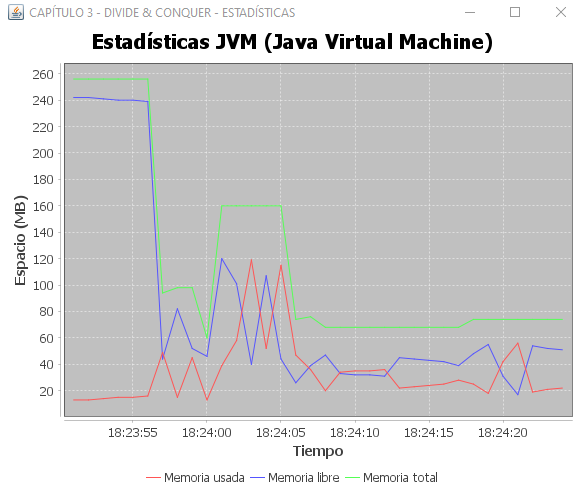
\includegraphics[width=\linewidth]{MVC/View/img/stats-jvm.png}
    \caption{Interfaz estadística JVM}
    \label{fig:Ejemplo stats JVM}
\end{figure}

\subsubsection{Estadísticas de los Algoritmos}\label{Stats Algt}

Este apartado de la vista principal, es el encargado de enseñar las estadísticas de la ejecución del algoritmo de los algoritmos ejecutados. Estas estadísticas incluyen una gráfica con el tiempo de ejecución de cada ejecución del algoritmo. Los resultados (tiempos de ejecución) son representados en un gráfico de barras, donde el eje \textit{x} representa el número de ejecuciones del algoritmo y el eje y el tiempo en milisegundos que ha tardado. Y finalmente, un gráfico de lineas con la evolución estimada de los tiempo de ejecución para la factorización de números primos, junto a su regreasión lineal.

\begin{figure}[!h]
    \centering
    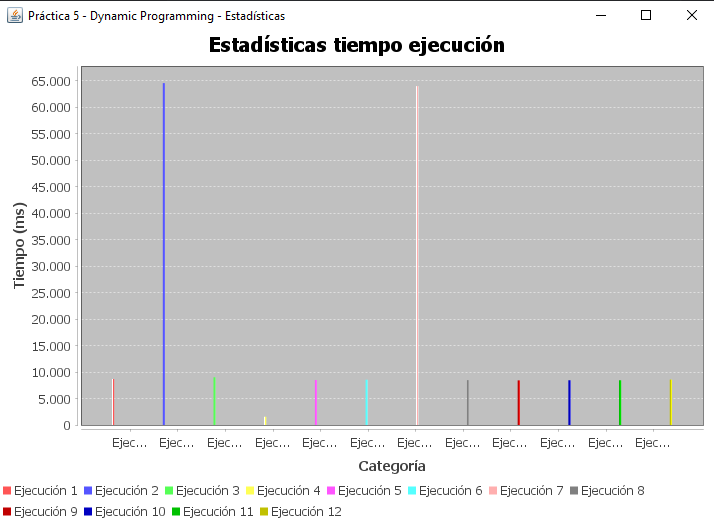
\includegraphics[width=\linewidth]{MVC/View/img/stats-algt.png}
    \caption{Interfaz estadísticas algortimos}
    \label{fig:Ejemplo stats Algt}
\end{figure}

Como se ha podido ver anteriormente en la imagen (\ref{fig:Ejemplo stats Algt}), se puede apreciar los diferentes datos obtenidos tras una serie de ejecuciones del algoritmo.
